
%(BEGIN_QUESTION)
% Copyright 2010, Tony R. Kuphaldt, released under the Creative Commons Attribution License (v 1.0)
% This means you may do almost anything with this work of mine, so long as you give me proper credit

Determine the temperature of the RTD, given a measured voltage of 89.2 millivolts between test points {\bf C} and {\bf D}, and 88.7 millivolts between test points {\bf E} and {\bf D}:

$$\includegraphics[width=15.5cm]{i00601x01.eps}$$

Assume a 100 $\Omega$ RTD with $\alpha = 0.00385$, and all wire resistances to be equal to each other.

\underbar{file i00601}
%(END_QUESTION)





%(BEGIN_ANSWER)

$V_{RTD}$ = 88.2 mV \hskip 30pt $V_{wire}$ = 0.5 mV (each current-carrying conductor)

\vskip 10pt

$R_{RTD}$ = 215.12 $\Omega$

\vskip 10pt

$T$ = 309 degrees Celsius (from table)

\vskip 10pt

$T$ = 299.02 degrees Celsius (from formula)

%(END_ANSWER)





%(BEGIN_NOTES)


%INDEX% Measurement, temperature: RTD (3-wire with cable resistance)

%(END_NOTES)

